\subsection{Induktive Ladung}\label{sec:energieuebertragung}

Der Dōjō wird mit Hilfe des Induktionsprinzips geladen. Der Ladeprozess wird gestartet, sobald der Dōjō auf die Ladestation gestellt wird. Beim Induktionsprinzip wird die Energie mithilfe von Spulen über eine kurze Distanz zwischen zwei Schaltungen transportiert. Die erste Schaltung, von welcher aus die Energie gesendet wird, wird Transceiver genannt. Diese Schaltung besteht aus einem Pulsgenerator, mit welchem das LC-Glied gepulst wird. Sie macht den Hauptanteil einer solchen Induktiven Ladeschaltung aus. Die zweite Schaltung, welche die Energie des Transceivers empfängt, wird Receiver genannt und besteht ebenfalls aus einem LC-Glied mit einem Gleichtrichter. Nachfolgend werden beide Teile der Schaltung beschrieben.

\subsubsection*{Tranceiver}
Der Pulsgenerator wird einer Timer-Schaltung umgesetzt. Verwendet wird hierbei das elektronische Bauelement NE555. Dieses bietet den Vorteil, dass das notwendige Pulssignal für die Übertragung einfach erstellt und verändert werden kann. Der NE555 enthält eine monolithisch integrierte Zeitgeberschaltung, die sich aufgrund ihrer Eigenschaften als Taktgeber, Oszillator und für Zeitverzögerungen verwenden lässt. Bevor der Timer zu schalten beginnt, müssen verschiedene Spannungsschwellen erreicht werden. Diese lassen sich durch extern angeschlossene Widerstände und Kondensatoren einstellen. Massgebend für die Veränderung der Pulsdauer, Frequenz und des Duty-Cycles sind die Verhältnisse der Komponenten. Das entstandene Pulssignal wird schlussendlich an das LC-Glied gegeben. Dafür wird das LC-Glied an die Versorgungsspannung gehängt und in Serie dazu der Collectoranschluss eines 2N3055 Leistungs NPN-Transistor angeschlossen. An dessen Emitter wird nun ein Niederohmiger Widerstand auf $GND$ gehängt, wobei die über ihm abfallenden Spannung von einem weiteren Transistor überwacht wird und somit den Strom begrenzt. Dieser \glqq 2N2222 Strombegrenzungs-Transistor\grqq wird zwischen dem Pulssignal, welches den Leistungs-Transistor steuert, und GND gehängt. Wird nun der Strom und somit auch die Spannung über dem Widerstand zu hoch, so schliesst der \glqq 2N2222 Strombegrenzungs-Transistor\grqq das Pulssignal kurz, wodurch der 2N3055 Leistungstransistor nicht mehr sauber durchgesteuert wird und dadurch den Strom begrenzt. Die Strombegrenzung ist abhängig von der verwendeten Peripherie des LC-Gliedes. Es gilt zu beachten, dass die Spule durch ihre kleine Bauform weniger Strom verträgt als der Leistungstransistor. In unserem Fall liegt der maximal zulässige Strom für die Spule bei $0.6A$. Bei der Wahl von grösseren Spulen muss jedoch darauf geachtet werden, dass die Begrenzung von 15A nicht überschritten wird, da dies die Belastungsgrenze für den 2N3055 Leistungstransistor ist.

\begin{figure}[H]
	\begin{center}
		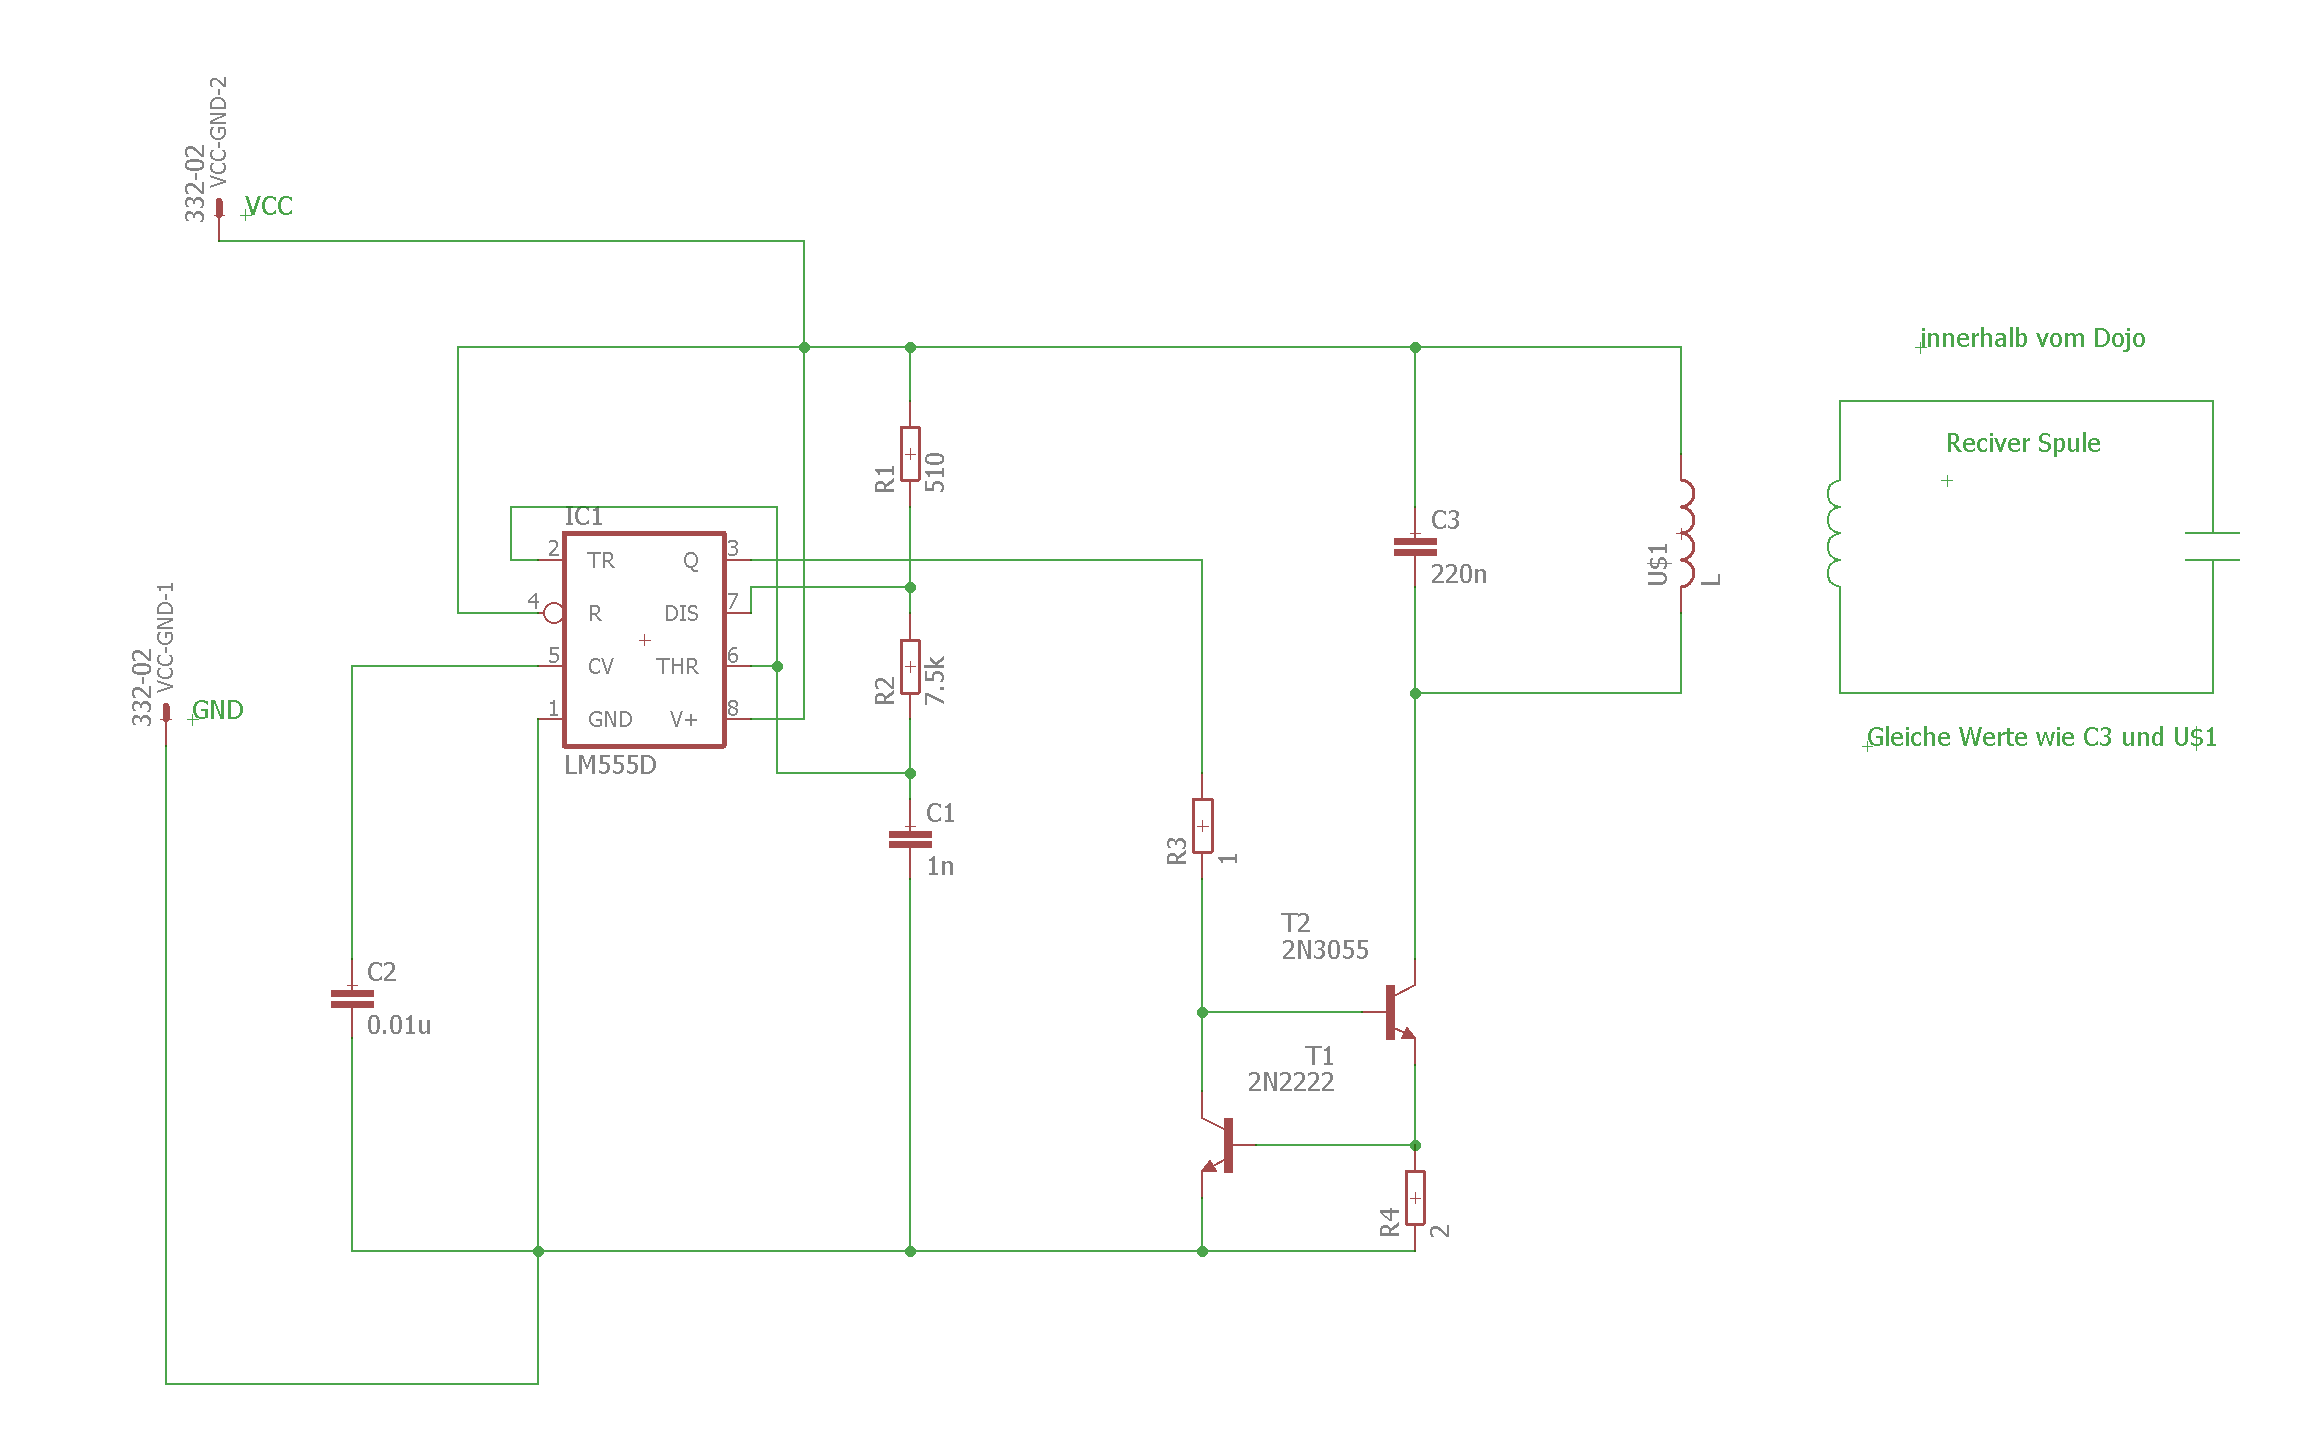
\includegraphics[width=80mm]{data/Tranceiver.png}
		\caption[Ne555]{Die verwendete Timerschaltung als Pulsquelle} %picture caption
		\label{fig:Tranceiver-Schaltung}
	\end{center}
\end{figure}
 
Das Pulssignal selber muss verschiedene Kriterien erfüllen. Zum einen sollte der Duty Cycle so nahe wie möglich an $50\%$ sein. Um dies zu erreichen muss $R2 >> R1$ gelten. Das andere Kriterium ist die Erreichung der Resonanzfrequenz des LC-Gliedes. Um das Pulssignal optimal einzustellen, können folgende Richtlinien betrachtet werden:
\begin{description}
	\item [$\cdot$ C] beeinflusst die Zeiten (Frequenz/High-Time/Low-Time)
	\item [$\cdot$ R$_{1}$] beeinflusst die High-Time, lässt jedoch die Low-Time unverändert.
	\item [$\cdot$ R$_{2}$ ] beeinflusst die High- und Low-Time und beeinflusst somit den Duty Cycle.
\end{description}

Die verwendeten Komponenten $C$, $R_{1}$ und $R_{2}$ wurden durch nachfolgende Formeln \ref{eq:TimerF} bis \ref{eq:TimerR2} berechnet. 

\begin{equation}\label{eq:Timerf}
f=1/T= 1.44/((R1+R2*2)*C)
\end{equation}
\begin{equation}\label{eq:TimerTL}
Low Time= 0.693*R*C
\end{equation}
\begin{equation}\label{eq:TimerTH}
High Time= 0.693*(R1+R2)*C
\end{equation}
\begin{equation}\label{eq:TimerDC}
D= Duty Cycle= (R1+R2)/(R1+2*R2)
\end{equation}
\begin{equation}\label{eq:TimerR1}
R1= 1.44**(2*D-1)/(F*C)
\end{equation}
\begin{equation}\label{eq:TimerR2}
R2= 1.44*(1-D)/(F*C)
\end{equation} 

Für die Berechnung der effektiven Werte, müssen die esten Werte angenommen werden. Unsere Berechnungen ergaben folgende für den Tranceiver am besten geeigneten Werte:

\begin{center}
C = $1nF$\\
R1 = $200\Omega$\\
R2 = $9k\Omega$\\
\end{center}
 
Die Frequenz (Formel \ref{eq:TimerF}) beträgt  $79.12kHz$. Nach der Berechnung der Komponenten folgt die Implementation in das Gerät. Es ist zu beachten, dass Abweichungen sich unmittelbar auf die Frequenz, die Pulsdauer und den Duty Cycle des Pulssignales auswirken. Eine solche Abweichung kann auch durch eine leicht abweichende Resonanzfrequenz des LC-Gliedes auftreten. In Kapitel \ref{sec:ladestation} wird ein Prototyp einer von uns entworfenen Ladestation vorgestellt, welche auch die gesamte Tranceiverschaltung implementiert.

Wie der Receiver aufgebaut ist, wird im nachfolgenden Abschnitt genauer erläutert.

\subsubsection*{Receiver}
Der Receiver besteht primär aus einem LC-Glied und einem Gleichrichter. Speziell ist, dass bei der Tranceiverschaltung das selbe LC-Glied verwendet wurde wie bei der Receiverschaltung. Dies aus dem Grund, weil das Energiefeld sehr klein ist und im Falle einer grösseren Spule das Receiver Glied nicht optimal ausgenutzt werden könnte. Das L-Glied (Flachspule) lässt sich mit einer Dimension von $\o 15mm$ Durchmesser und $2mm$ Höhe gut im inneren des Dōjō’s platzieren. Die Positionierung findet am Boden statt und ermöglicht dadurch die besten Übertragungswerte von Strom und Spannung. Der notwendige Kondensator für die Vervollständigung des LC-Gliedes kann direkt hinter der Spule montiert werden. Die hochfrequente Wechselspannung welche nun gemessen werden kann, muss für die Speisung der Batterie noch gleichgerichtet werden. Verwendet werden hierbei sowohl Kondensatoren als auch spezielle Gleichrichterdioden, welche eine Abfallspannung von lediglich $0.1V$ aufweisen. Anschliessend wird die gesamte Ladeschaltung gespiesen, welche den gesamten Ladeprozess des Akkus übernimmt. Einen Einblick in diesen Ladeprozess gibt nachfolgendes Kapitel.
